\documentclass[a4paper,11pt,oneside]{report}
\usepackage[latin1]{inputenc}
\usepackage{calc}
\usepackage[dvips]{graphicx}
%\DeclareGraphicsExtensions{.pdf}
\usepackage[english]{babel}
\usepackage[T1]{fontenc}
\usepackage{booktabs}
\usepackage{setspace}
%\usepackage{indentfirst}

\usepackage {amsmath, amssymb}
% \usepackage{biblatex}
\usepackage{float} 
\usepackage{bbold}
\usepackage{mathbbol}
\usepackage{amsmath}
\usepackage{amsfonts} 
\usepackage{verbatim}
\usepackage{graphicx}
\usepackage{tikz-cd}
\usepackage{amsthm}

\usetikzlibrary{arrows}
\usetikzlibrary{matrix}



\newtheorem{teor}{Theorem}[chapter] 
\newtheorem{defi}[teor]{Definition}
\newtheorem{oss}[teor]{Remark}
\newtheorem{prop}[teor]{Proposition}
\newtheorem{lemma}[teor]{Lemma}
\newtheorem{coroll}[teor]{Corollary}
\newtheorem{es}{Example}[chapter]





\newcommand{\de}{\partial}
\newcommand{\gp}{\ensuremath{\pi_{n}(X,x_{0})}}
\newcommand{\fne}{\ensuremath{f: X \rightarrow Y}}
\newcommand{\gpr}{\ensuremath{\pi_{n}(X,A,x_{0})}}
\newcommand{\virg}[1]{``#1''}
\newcommand{\s}{\star}
\newcommand{\riga}{\bigskip }
\newcommand{\e}{ \omega_{x_0}}
\newcommand{\ey}{ \omega_{y_0}}
\newcommand{\p}{p_{\ast}}
\newcommand{\cc}{\ensuremath{\mathbb{C}}}
\newcommand{\zz}{\ensuremath{\langle z_1,z_2 \rangle}}
\newcommand{\z}{\ensuremath{\mathbb{Z}}}
\newcommand{\q}{\ensuremath{\mathbb{H}}}




\graphicspath{ {img/} }

\title{First Assignment Multivariate Statistical Analysis}
\author{Claudio Peroni}
\date{}

\begin{document}
\maketitle

\section*{Exercise 1}
\subsection*{1.1)}
	We begin by taking the log transformation of the variables $x_2$, $x_3$, $x_4$.
	From now on we will refer to the logarithm of the variables using the name of the variables themselves.

\subsection*{1.2)}
	We compute the sample mean, variance and correlation of the variables using the built-in R commands.

	\begin{align}
	\mu &= 
	\begin{bmatrix}
	  1.121 \\ 
	  4.263 \\ 
	  3.244 \\ 
	   \end{bmatrix}\\
	S &=
	\begin{bmatrix}
	  0.525 & 0.003 & 0.086 \\ 
	  0.003 & 0.012 & -0.013 \\ 
	  0.086 & -0.013 & 0.091 \\ 
	   \end{bmatrix}\\
	R &= \begin{bmatrix}
	  1.000 & 0.043 & 0.393 \\ 
	  0.043 & 1.000 & -0.400 \\ 
	  0.393 & -0.400 & 1.000 \\ 
	   \end{bmatrix}
	\end{align}
	The first thing we notice in the matrix of the variances and covariances $S$ is that the variance of $x_2$ is greater by one order of magnitude than the other two variances.
	By looking at the correlation matrix $R$ we note that the correlation between $x_2$ and $x_4$ is almost the same of the one between $x_3$ and $x_4$ (in absolute value), while the correlation between $x_2$ and $x_3$ is almost negligible.
\subsection*{1.3)}
	First we plot the boxplot of all the variables together. This graph shows that the range of the variables is quite different. Then we plot the boxplot of each variable separately in order to highlight the outliers.
	We find that both the second and the third variable have one outlier each. They are respectively the 34th and 47th observation. It appears that there is no univariate outlier for the first variable.
	\begin{figure}[H]
	\centering
	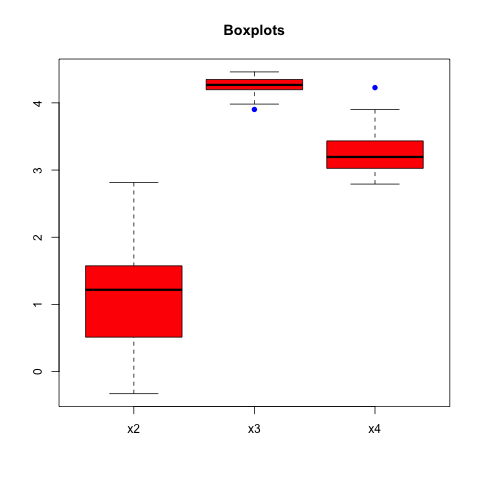
\includegraphics[width=10cm, height=8cm]{boxplot_same_scale.png}
	\caption{The boxplot of the variables. Outliers in blue.}
	\end{figure}
	\begin{figure}[H]
	\centering
	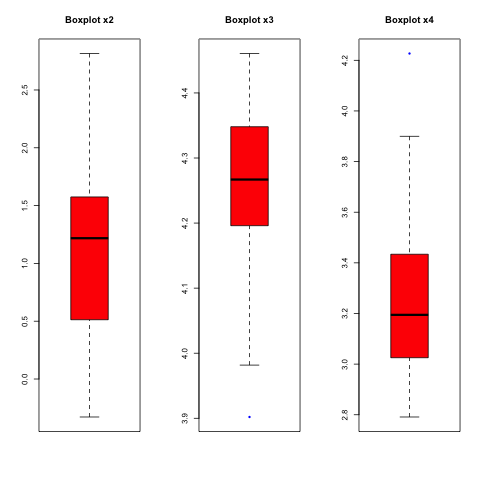
\includegraphics[width=10cm, height=8cm]{boxplots.png}
	\caption{The boxplots for each variable separately. Outliers always in blue.}
	\end{figure}

\subsection*{1.4)}
	\begin{figure}[H]
	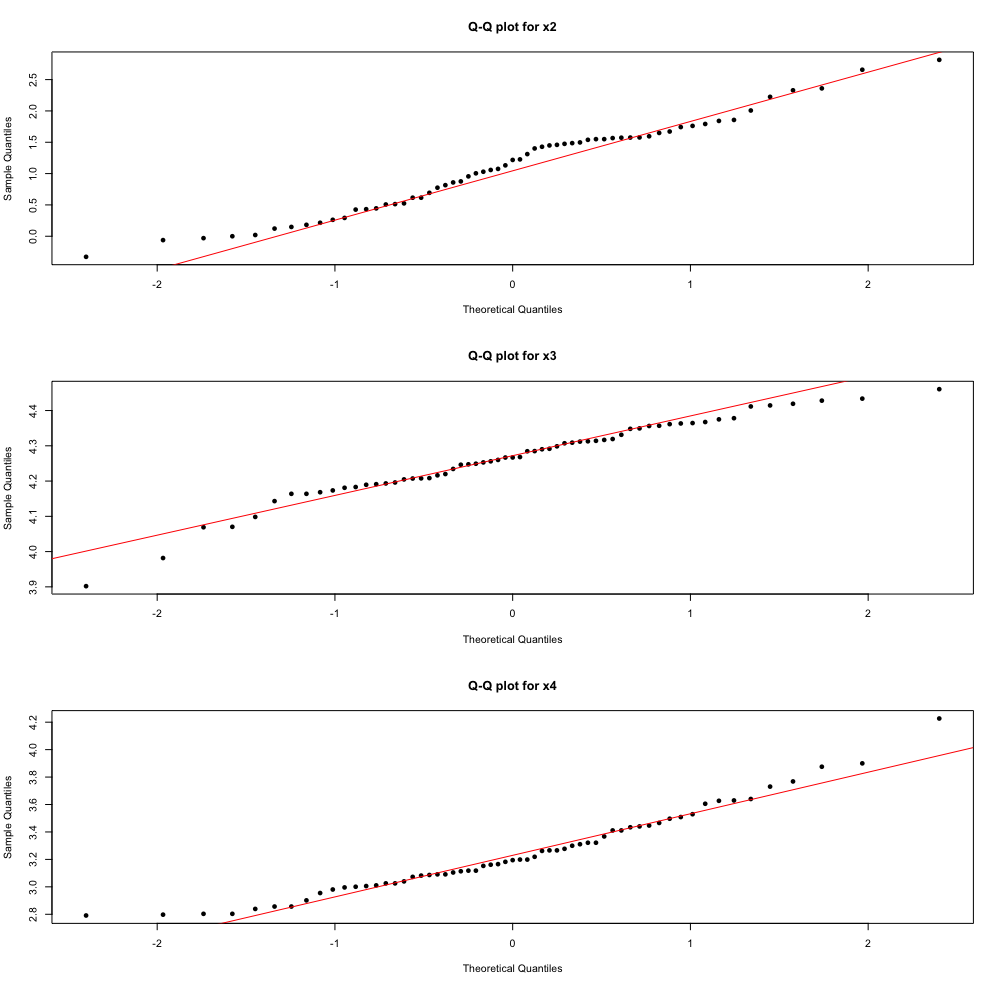
\includegraphics[width = 15cm, height = 19cm]{q_qplot_ex1.png}
	\caption{Q-Q plots for the variables.}
	\end{figure}
	A visual inspection of the normal Q-Q plots leads us not to reject the univariate normality hypothesis. We notice that there is a slightly unexpected behaviour at the tails.
	
\subsection*{1.5)}
	
	\begin{figure}[H]
	\centering
	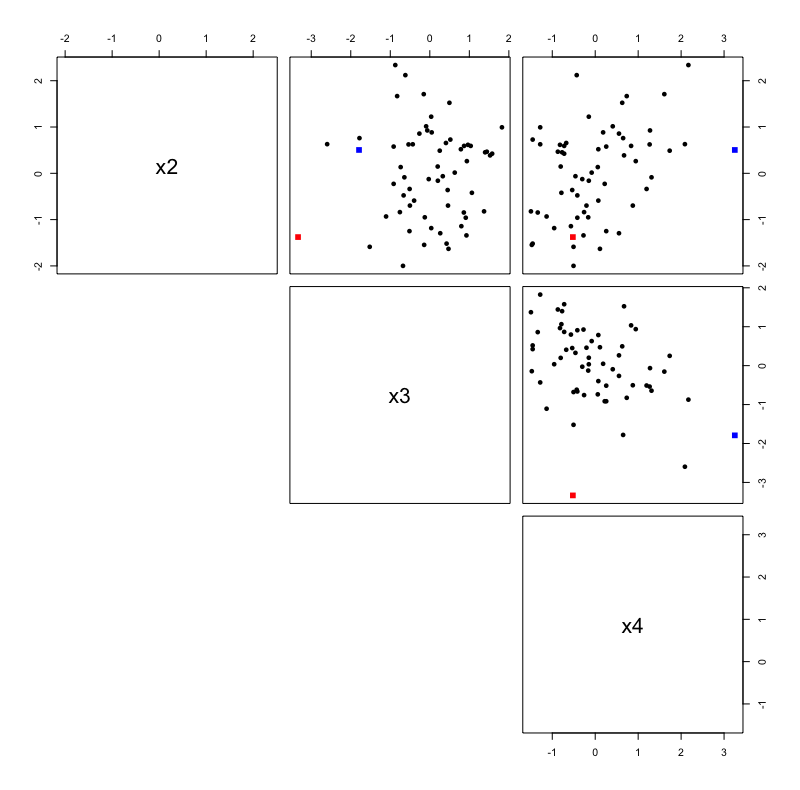
\includegraphics[scale = 0.5]{pairs_scatterplot1_ex1.png}
	\caption{Scatterplots for the variables. In blue the outlier for $x_4$ and in red the outlier for $x_3$.}
	\end{figure}
	The univariate outliers we found for $x_3$ and $x_4$ are still visible in the bivariate representation of the scatterplots when the variable for which they are univariate outliers is plotted against another.

\subsection*{1.6)}
	To compute the squared Mahalanobis distance $d^2$ we use the formula:
	\begin{align}
	d^2 = (x_i - \bar x)^T \mathbf{S}^{-1} (x_i - \bar x)
	\end{align}
	The result is:
	\begin{figure}[H]
	\verbatiminput{"codeverbatim/Mahalanobis.txt"}
	\caption{the output of the $d^2$ vector in the R console.}
	\end{figure}

\subsection*{1.7)}
	\begin{figure}[H]
	\centering
	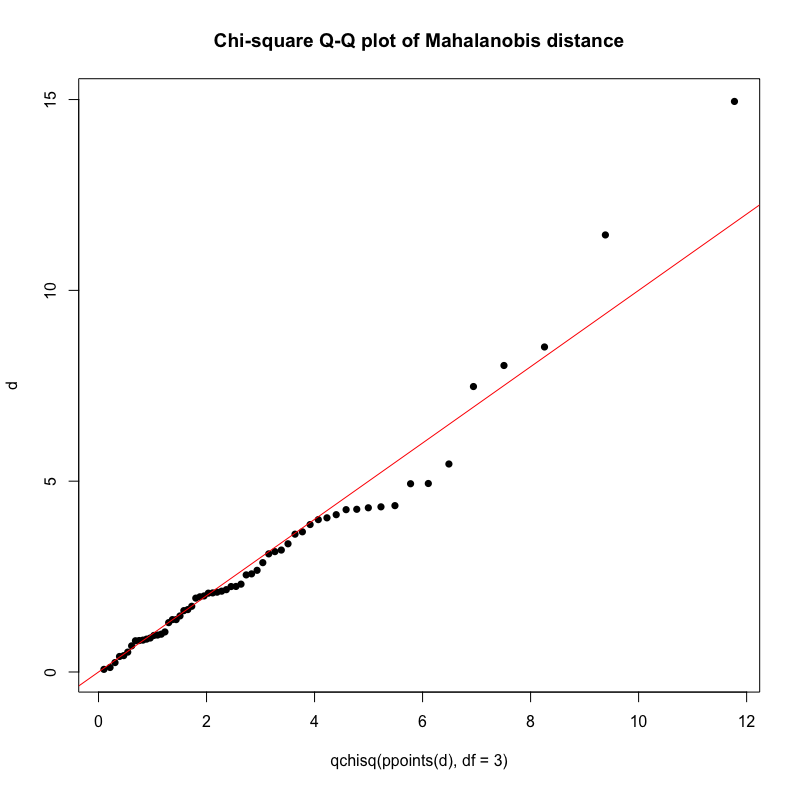
\includegraphics[scale = 0.35]{Mahala_q_q_chi.png}
	\caption{Chi-squared Q-Q plot of the $d^2$ distance.}
	\end{figure}
	This plot shows that the $d^2$ distances follow the q-q line quite strictly except the last two. Hence we do not reject normality of the data.
	
\subsection*{1.8)}
	To find other candidates outliers we sort the $d^2$ distances and look for unusually large or small values.
	\begin{figure}[h]
	\centering
	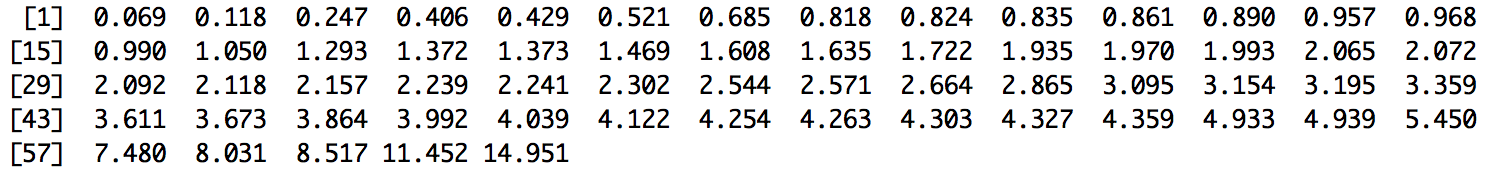
\includegraphics[scale = 0.55]{sorted_d.png}
	\caption{The sorted $d^2$ distances.}
	\end{figure}
	We see that 5 observations present unusually large distances. They are the 6th, 34th, 47th, 48th, 49th observations. We had already classified as outliers two of them (the 34th and 47th) during the univariate analysis.
	In order to visualise these 3-dimensional outliers we use a 3D-scatterplot. Here we have coloured all the 5 outliers found.
	\newline
	\begin{figure}[h]
	\centering
	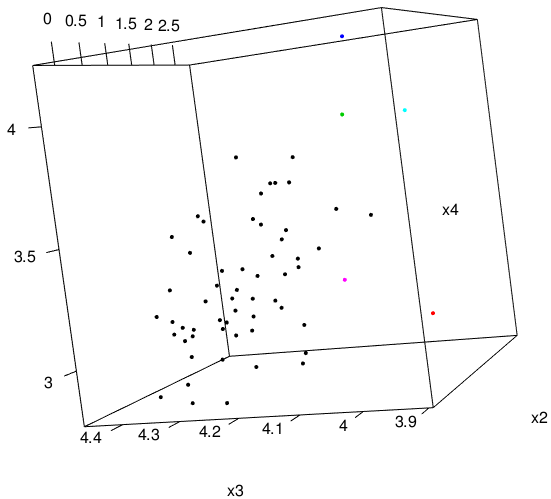
\includegraphics[scale = 0.55]{3dplot1.png}
	\caption{3D scatterplot of the data.}
	\end{figure}
	\begin{figure}[H]
	\centering
	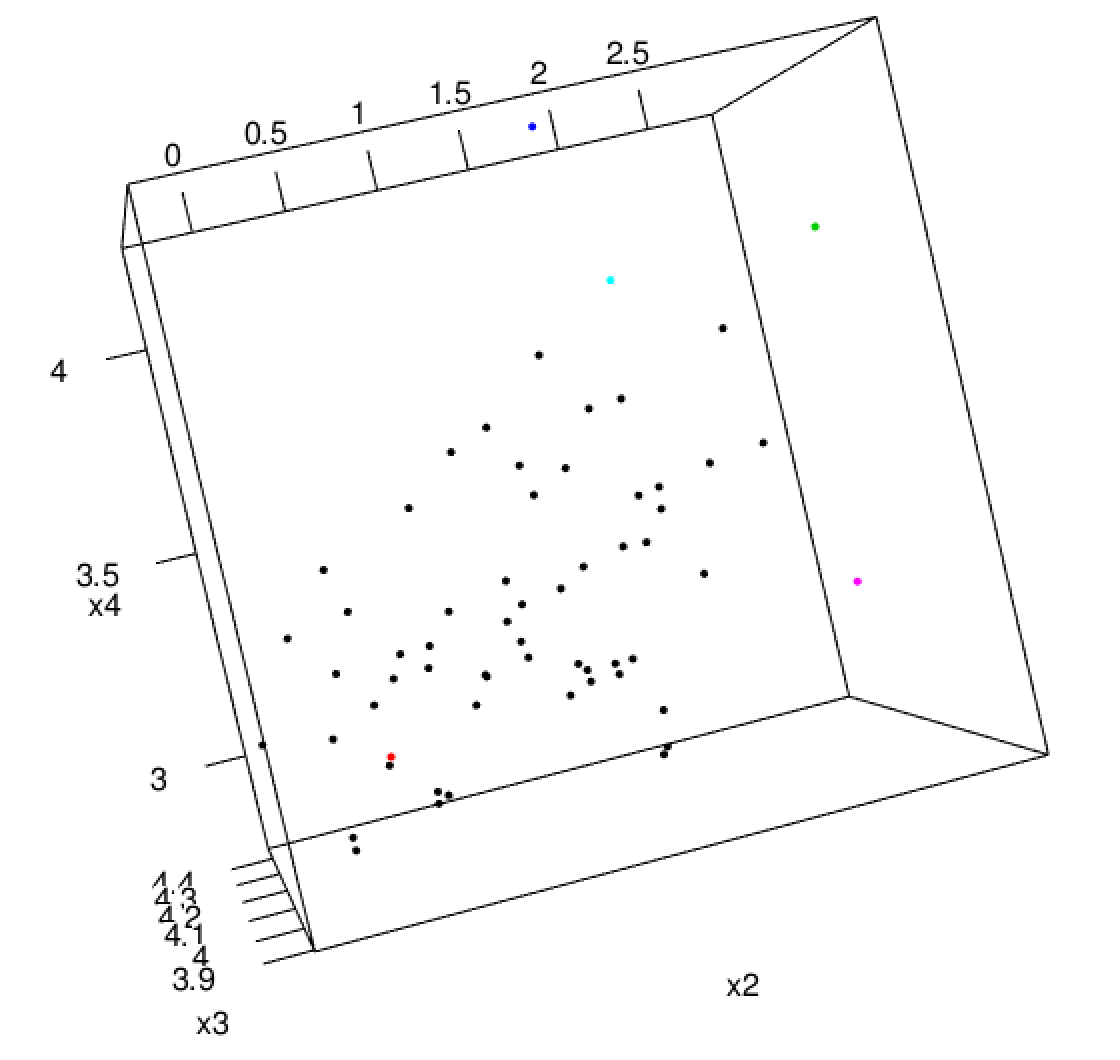
\includegraphics[scale = 0.55]{3dplot2.png}
	\caption{3D scatterplot of the data from a different perspective.}
	\end{figure}

\newpage
\section*{Exercise 2}
\subsection*{2.1)}
	We have to compute the distribution of $X_3|(X_1, X_2) = (x_1, x_2)$.
	In order to do so, we apply the following general formulas:
	\begin{align}
		\bar \mu &= \mu_1 + \Sigma_{12} \Sigma_{22}^{-1}(a - \mu_2) \label{eq:cond_mean} \\
		\bar \Sigma &= \Sigma_{11} - \Sigma_{12} \Sigma_{22}^{-1} \Sigma_{21} \label{eq:cond_Sigma}
	\end{align}
	to our case (where $a = (x_1, x_2)$). The result is:
	\begin{align}
		\bar \mu_3 &= 2 - \frac{1}{2}x_1 - \frac{1}{2}x_2\\
		\bar \Sigma_3 &= \frac{3}{4}
	\end{align}
	Therefore, we conclude that $X_3|(X_1, X_2) = (x_1, x_2)$ is distributed as a normal with mean $\bar \mu_3$ and variance $\bar \Sigma_3$.
	
\subsection*{2.2)}
	Again we use (\ref{eq:cond_mean}) and (\ref{eq:cond_Sigma}) to compute the distribution of $$(X_1, X_2)|X_3 = x_3 = 0$$
	We get:
	\begin{align}
		\bar \mu_{12} &= \left(\frac{3}{2}, -\frac{1}{2} \right)\\
		\bar \Sigma_{12} &= 
			\begin{bmatrix}
	  			\dfrac{15}{16} & -\dfrac{9}{16}\\[2ex]
	 			-\dfrac{9}{16} & \dfrac{15}{16}\\[2ex]
	  		\end{bmatrix}
	\end{align}
	Once more, we conclude that $(X_1, X_2)|X_3 = x_3 = 0$ is distributed as $N(\bar \mu_{12}, \bar \Sigma_{12})$.
	Then, we sketch the ellipse $$ (x - \bar \mu_{12})^T \bar \Sigma_{12}^{-1} (x - \bar \mu_{12}) = \chi^{2}_{2,\alpha}$$
	In the 2-dimensional space $x = (x_1, x_2)$ for $\alpha = 0.1$.
	
	\begin{figure}[H]
	\centering
	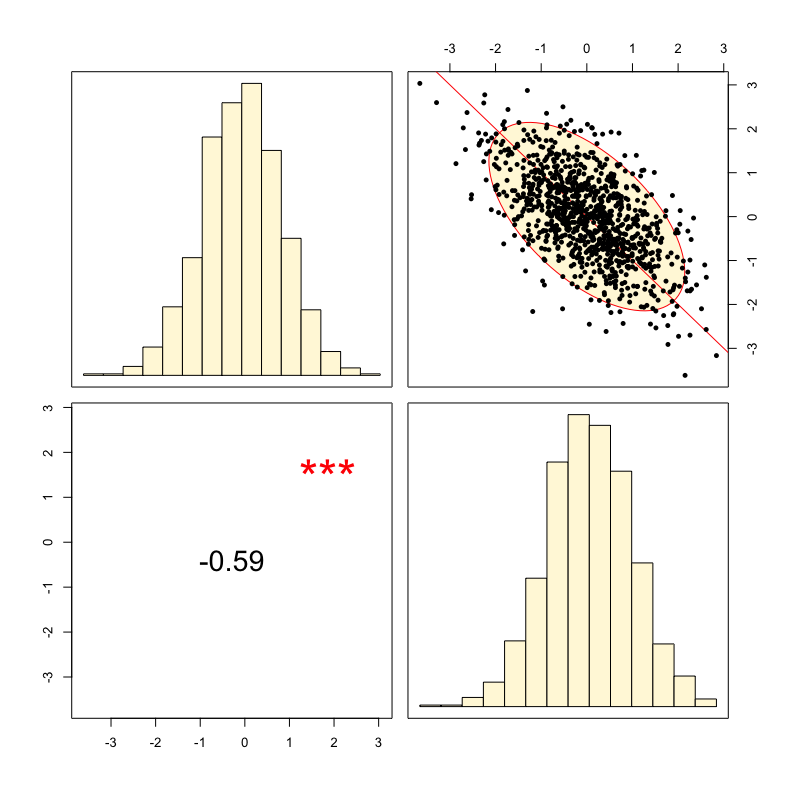
\includegraphics[scale = 0.55]{pairs_ellipse.png}
	\caption{Scatterplot of data with ellipse (of level $\alpha = 0.1$), univariate histograms, and correlation between the variables.}
	\end{figure}

\newpage
\section*{Exercise 3}
\subsection*{3.1)}
	We perform the Principal Component Analysis on the standardised variables of the \textit{socio} dataset. The result is the following:
	\begin{figure}[H]
	\centering
	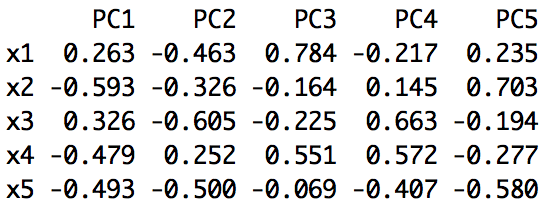
\includegraphics[scale = 0.8]{PCA_socio.png}
	\caption{Rotation matrix.}
	\label{fig:rot}
	\end{figure}
	Each columns contains the coefficients of the linear combination of the original variables for each Principal Component.

\subsection*{3.2)}
	\begin{figure}[H]
	\centering
	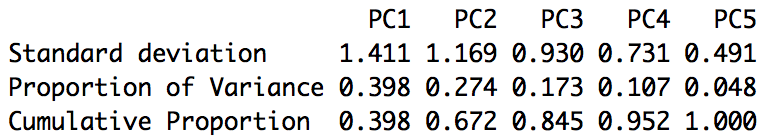
\includegraphics[scale = 0.8]{importance_pca.png}
	\caption{The \textit{importance matrix} of the principal components.}
	\end{figure}
	The cumulative proportion of variance explained by the first two PCs is $0.672$.

\subsection*{3.3)}
	\begin{figure}[H]
	\centering
	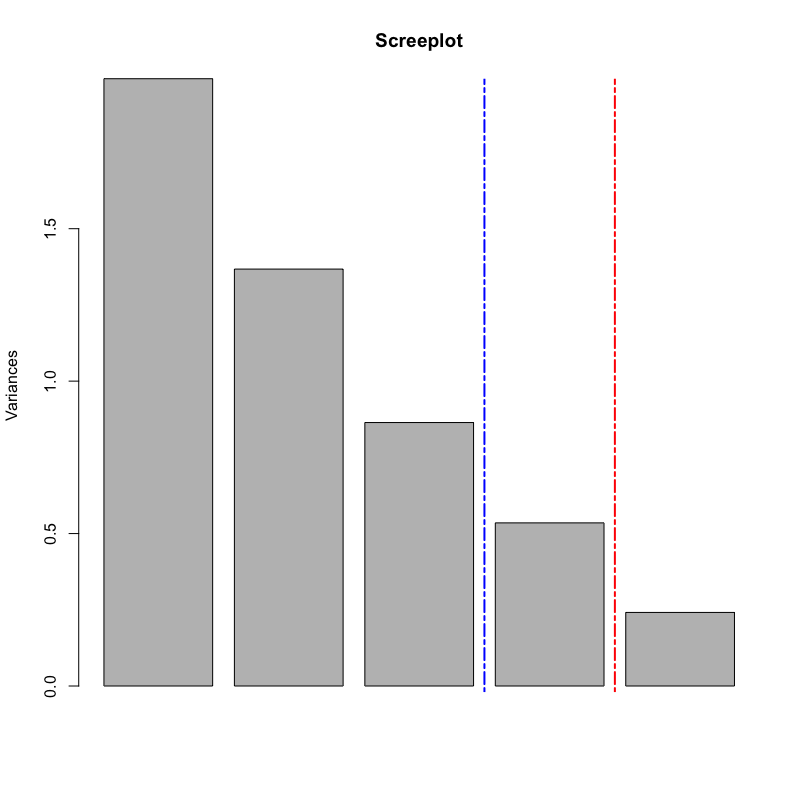
\includegraphics[height = 11cm, width = 15cm]{screeplot_bar.png}
	\caption{Screeplot (type "barplot") of the PCs. In blue and red the suggested tresholds.}
	\end{figure}
	From the screeplot and the importance matrix we can see that 3 PCs are enough to explain more than 80\% of the variance. For many uses this is probably enough. If we add one more PC, we are able to account for $\sim95\%$ of the total variance, so in some cases this might be the best choice.
\subsection*{3.4)}
	First we retrieve the PCA results from Lecture 4.
	\begin{figure}[H]
	\centering
	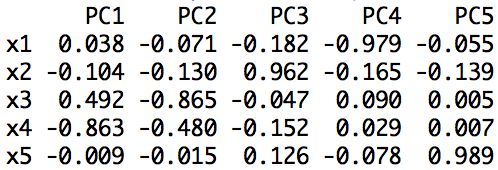
\includegraphics{pca_De_Blasi.png}
	\caption{Principal Component rotation matrix from Lecture 4 as comparison. Here data are \textit{not} standardised.}
	\end{figure}
	This rotation matrix suggests that the first component can be seen as an explanatory variable for $x_4$, while the second principal component for $x_3$ (and a similar relation can be found between the other 3 PCs with the remaining variables). The link between each PC and one of the original variables is more evident here than in our analysis, see Figure \ref{fig:rot}.
	\begin{figure}[H]
	\centering
	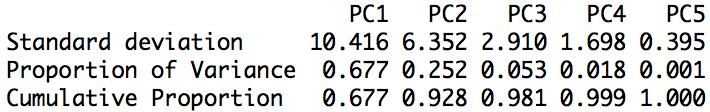
\includegraphics{pca_De_Blasi_importance.png}
	\caption{The \textit{importance matrix} of the principal components from PCA in Lecture 4.}
	\end{figure}
	\begin{figure}[H]
	\centering
	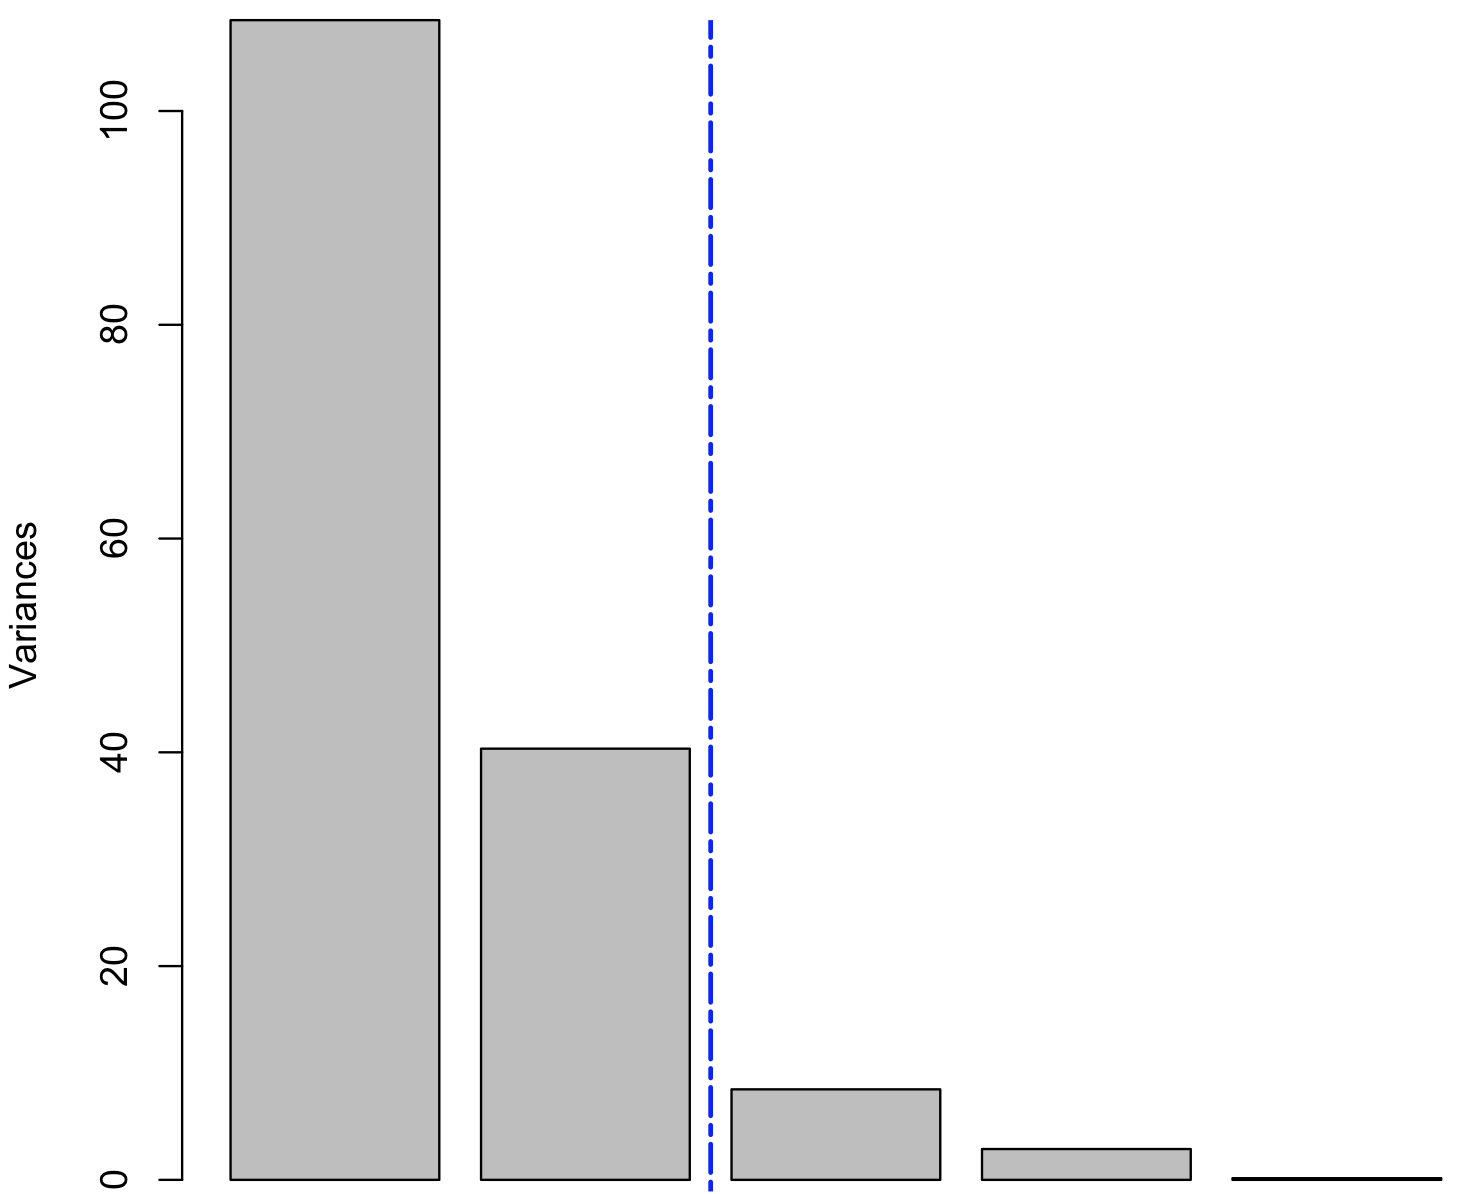
\includegraphics[height = 8cm, width = 13cm]{screeplot_bar_De_Blasi.png}
	\caption{A Graphical visualisation of the cumulative proportion of variance explained bye the PCs (bar screeplot). In blue the obvious cutoff.}
	\end{figure}
	
	Concerning the Cumulative Proportion explained by the Principal Components, we see that the first two PCs are enough to account for more than 90\% of the total variance, while in our analysis we need 4 PCs to reach a similar explanation proportion.
	This difference is due to the standardisation of our data. With non-standardised data the variables which have greater variance tend to \textit{weigh} more in the cumulative proportion.

	
\end{document}